\section{Solve - The modulus iteration algorithm} \label{sec_solve}
The last function, that had to be implemented was a solver for a PL function in abs-normal form. Given:
\begin{flalign*}
	a,b,Z,L,J,Y,m,n,\Delta y
\end{flalign*}
We want to calculate:
\begin{flalign*}
	\Delta x, \Delta z
\end{flalign*}

\subsection{Deducing a solution}
In \cite{Griewank2017} Multiple solutions with different properties in convergence and complexity have been suggested. Here we focus on the algorithm that in \cite{Griewank2017} is called modulus iteration algorithm. \\
For deducing this algorithm we first and foremost assume:
\begin{flalign*}
	\Delta y = 0
\end{flalign*}
If this condition is not fulfilled, we can replace $b$ with $b'$:
\begin{flalign*}
	b' = b - \Delta y
\end{flalign*}
and replace $\Delta y$ with the zero-vector $O_m$. Now we can rearrange the equation system:
\begin{flalign*}
	\Delta y &= b + J \Delta x + Y |\Delta z| \\
	0 &= b + J \Delta x + Y |\Delta z| \\
	- b - Y |\Delta z| &= J \Delta x \\
	b + Y |\Delta z| &= J \Delta x (-1) \\
	J^{-1}(b + Y |\Delta z|) &= - \Delta x
\end{flalign*}
and obtain:
\begin{flalign}
	\Delta x = - J^{-1}(b + Y |\Delta z|) \label{eq_modulus_dx}
\end{flalign}
For calculating $\Delta z$ we can now use (\ref{eq_modulus_dx}):
\begin{flalign*}
	\Delta z &= a + Z \Delta x + L |\Delta z| \\
	&= a + Z \Big( - J^{-1}(b + Y |\Delta z|) \Big) +  L |\Delta z| \\
	&= a + Z \Big( -J^{-1}b - J^{-1}Y|\Delta z| \Big) +  L |\Delta z| \\
	&= a - ZJ^{-1}b - Z J^{-1}Y|\Delta z| +  L |\Delta z| \\
	&= a - ZJ^{-1}b - (Z J^{-1}Y - L)|\Delta z| \\
\end{flalign*}
Summarized:
\begin{flalign}
\Delta z &= c + S|\Delta z| \label{eq_modulus} \\
c		 &= a - ZJ^{-1}b \label{eq_c} \\
S		 &= L - Z J^{-1}Y \label{eq_S}
\end{flalign}

We can use this result to construct a fix-point iteration algorithm where we recalculate $\Delta z$ in each step until convergence. In the following we focus onto the implementation of this algorithm.

\subsection{Implementation}
Implementing this algorithms means calculating (\ref{eq_c}) and (\ref{eq_S}) once and using these to repeatedly calculate (\ref{eq_modulus}).
The key problem here is the calculation of $J^{-1}$, since this is the most expensive Operation. We decided to do a QR-decomposition of $J = QR$ and solving the linear equation system instead of calculating $J^{-1}$ directly. E.g. calculating $c$ is done in the following way:

\begin{enumerate}
	\item $J = QR$
	\item Solve $b = QRx$
		\begin{flalign*}
			QR x &= b \\
			x    &= solve(Rx = Qb)
	\end{flalign*}
	\item Calculate $c$:
	\begin{flalign*}
		c = a - Zx
	\end{flalign*}
\end{enumerate}
The calculation of $S$ follows the same  pattern. After convergence $\Delta x$ can be calculated according to (\ref{eq_modulus_dx}).

\subsection{Performance Experiment}
We implemented a serial version in numpy and a parallel version in CUDA C++, but in the following we focus on the CUDA implementation.
We did an experiment to benchmark the performance of our implementation. Obviously this only made sense as long as the results were correct. To verify this, we preceded as follows:
\begin{enumerate}
	\item Randomly generate a function in abs-normal form: $a,b,Z,L,J,Y, \Delta x$ according to (\ref{absnf}).
	\item Evaluate given function to obtain: $\Delta y$ and $\Delta z$
	\item Solve the system for $\Delta x$ and $\Delta z$ with the results of the previous step
	\item Verify if the resulting $\Delta x$ and $\Delta z$ match the original ones.
\end{enumerate}

We measured the runtime of the solve function in given context. To make sure, that each device works with the same data, we fixed the seed for the pseudo-random number generator. The results of this experiment can be found in fig \ref{fig_modulus_runtime}. 

\begin{figure}[ht]
	\centering
	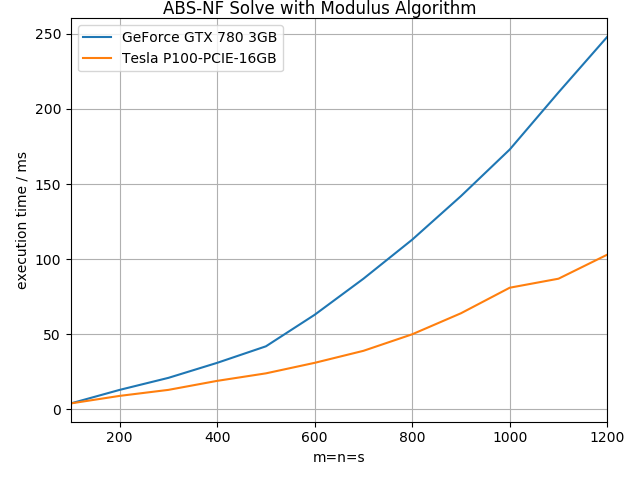
\includegraphics[width=0.6\textwidth]{img/solve_modulus.png}
	\caption{Runtime of the modulus solve implementation}
	\label{fig_modulus_runtime}
\end{figure}

\subsection{Analysis and Notes}
The implementation works correctly and the runtime results in fig. \ref{fig_modulus_runtime} behave as expected. We did not include the runtime of the serial version on purpose. This was for two reasons:
\begin{enumerate}
	\item The numpy implementation calculates the inverse of $J$ directly.
	\item We had to make sure, that each version operates on the exact same data, which we didn't
\end{enumerate}

